%%%%%%%%%%%%%%%%%%%%%%%%%%%%%%%%%%%%%%%%%
% Journal Article
% LaTeX Template
% Version 1.4 (15/5/16)
%
% This template has been downloaded from:
% http://www.LaTeXTemplates.com
%
% Original author:
% Frits Wenneker (http://www.howtotex.com) with extensive modifications by
% Vel (vel@LaTeXTemplates.com)
%
% License:
% CC BY-NC-SA 3.0 (http://creativecommons.org/licenses/by-nc-sa/3.0/)
%
%%%%%%%%%%%%%%%%%%%%%%%%%%%%%%%%%%%%%%%%%

%----------------------------------------------------------------------------------------
%	PACKAGES AND OTHER DOCUMENT CONFIGURATIONS
%----------------------------------------------------------------------------------------

\documentclass[twoside,twocolumn]{article}

\usepackage{blindtext} % Package to generate dummy text throughout this template 

\usepackage[sc]{mathpazo} % Use the Palatino font
\usepackage[T1]{fontenc} % Use 8-bit encoding that has 256 glyphs
\linespread{1.05} % Line spacing - Palatino needs more space between lines
\usepackage{microtype} % Slightly tweak font spacing for aesthetics

\usepackage[english]{babel} % Language hyphenation and typographical rules

\usepackage[hmarginratio=1:1,top=32mm,columnsep=20pt]{geometry} % Document margins
\usepackage[hang, small,labelfont=bf,up,textfont=it,up]{caption} % Custom captions under/above floats in tables or figures
\usepackage{booktabs} % Horizontal rules in tables

\usepackage{lettrine} % The lettrine is the first enlarged letter at the beginning of the text

\usepackage{enumitem} % Customized lists
\setlist[itemize]{noitemsep} % Make itemize lists more compact

\usepackage{abstract} % Allows abstract customization
\renewcommand{\abstractnamefont}{\normalfont\bfseries} % Set the "Abstract" text to bold
\renewcommand{\abstracttextfont}{\normalfont\small\itshape} % Set the abstract itself to small italic text

\usepackage{titlesec} % Allows customization of titles
\renewcommand\thesection{\Roman{section}} % Roman numerals for the sections
\renewcommand\thesubsection{\roman{subsection}} % roman numerals for subsections
\titleformat{\section}[block]{\large\scshape\centering}{\thesection.}{1em}{} % Change the look of the section titles
\titleformat{\subsection}[block]{\large}{\thesubsection.}{1em}{} % Change the look of the section titles

\usepackage{fancyhdr} % Headers and footers
\pagestyle{fancy} % All pages have headers and footers
\fancyhead{} % Blank out the default header
\fancyfoot{} % Blank out the default footer
\fancyhead[C]{Harvey Hughes $\bullet$ October 2018 $\bullet$ Emmanuel College} % Custom header text
\fancyfoot[RO,LE]{\thepage} % Custom footer text

\usepackage{titling} % Customizing the title section

\usepackage{hyperref} % For hyperlinks in the PDF

\usepackage{graphicx}
\graphicspath{ {images/} }

\newenvironment{reusefigure}[2][htbp]
  {\addtocounter{figure}{-1}%
   \renewcommand{\theHfigure}{dupe-fig}% If you're using hyperref
   \renewcommand{\thefigure}{\ref{#2}}% Figure counter is \ref
   \renewcommand{\addcontentsline}[3]{}% Avoid placing figure in LoF
   \begin{figure}[#1]}
  {\end{figure}}
\usepackage{wrapfig}
\usepackage{amsmath}
%----------------------------------------------------------------------------------------
%	TITLE SECTION
%----------------------------------------------------------------------------------------

\setlength{\droptitle}{-4\baselineskip} % Move the title up

\pretitle{\begin{center}\Huge\bfseries} % Article title formatting
\posttitle{\end{center}} % Article title closing formatting
\title{Random variables and random number generation } % Article title
\author{%
\\
\textsc{Harvey Hughes} \\
\normalsize Emmanuel College \\ % Your institution
\normalsize Lab Date : 17/10/18\\
\normalsize \href{mailto:hh458@cam.ac.uk}{hh458@cam.ac.uk} % Your email address
}
\date{\today} % Leave empty to omit a date
\renewcommand{\maketitlehookd}{%
\begin{abstract}
\noindent
The purpose of this lab was to introduce random variables and how transformations can be used to generate a different probability density. This would be achieved using Matlab to back up theoretical results of random variables. Jacobian, inverse CDF and non linear transformations were investigated. The theory agreed with Matlabs random number generation throughout.
\newline
\end{abstract}
}

%----------------------------------------------------------------------------------------

\begin{document}

% Print the title
\maketitle

%----------------------------------------------------------------------------------------
%	ARTICLE CONTENTS
%----------------------------------------------------------------------------------------

\section{Introduction}

\lettrine[nindent=0em,lines=3]{D}uring the course of the lab various methods and techniques were used to generate distributions of random variables using Matlab.
\newline
With the objectives being:
\begin{itemize}
\item Introduce the idea of random variables and functions of them\\
\item To use the Jacobian to transform random variables\\
\item To experiment with non uniform random number generation\\
\end{itemize}

%------------------------------------------------


\section{Results and Discussion}
\subsection{1. Uniform and normal random variables}
\begin{figure}[h]
  \centering
    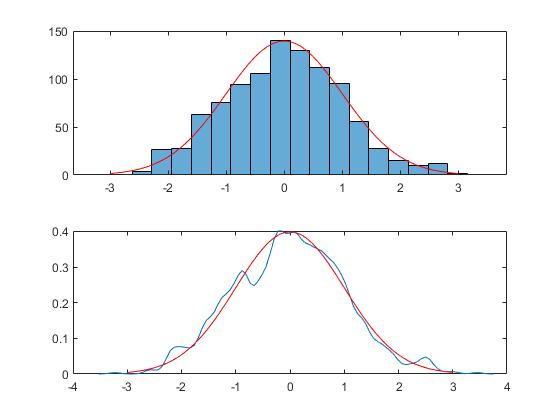
\includegraphics[width=\linewidth]{1normal}
  \caption{Histogram and kernel density plot using a Gaussian kernel $\mathcal{N}(0,1)$ with sample size 1000}
  \label{fig:1normal}
\end{figure}
\begin{figure}[h]
  \centering
    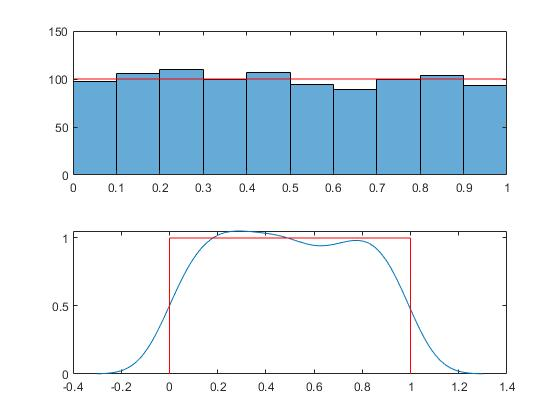
\includegraphics[width=\linewidth]{1uniform}
  \caption{Histogram and kernel density plot using a uniform distribution $\mathcal{U}(0,1)$ with sample size 1000}
  \label{fig:1uniform}
\end{figure}

When a Gaussian kernel is used, as in figure \ref{fig:1normal}, it is clear that a kernel density method to approximate the distribution leads to a more accurate curve. This is due to the smoothing inherent in the kernel density method which removes the jaggedness that is shown in the histogram plot.

The opposite is true for distributions with a large discontinuity in density function such as a uniform distribution pictured in figure \ref{fig:1uniform}. This figure shows the smoothing present with the kernel method either side of the bounds [0,1]. This leads to an incorrect shape of density function. The histogram plot more accurately depicts the distribution due to bin height tending towards the mean as N increases and therefore all bin heights being close to the pdf.

\begin{figure}[h]
  \centering
    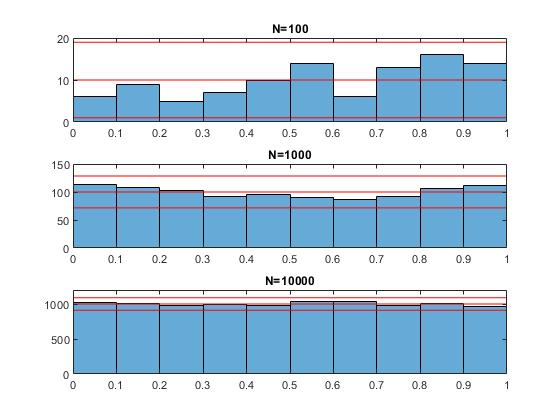
\includegraphics[width=\linewidth]{1means}
  \caption{Histogram plots using a uniform distribution $\mathcal{U}(0,1)$, showing how the theoretical mean and $\pm3\sigma$ of bin height varies with sample size}
  \label{fig:1means}
\end{figure}

\begin{equation}
\label{eq:1meancal}
\begin{split}
&\mu = Np_{j}\\
&\sigma^2=Np_j(1-p_j)\\
\end{split}
\end{equation} 

The theoretical mean and standard deviation of bin height in histogram plots can be calculated using equations \ref{eq:1meancal}. These values have been calculated and plotted in figure \ref{fig:1means} for three different sample sizes from a uniform distribution. $P_j$ is the probability of the distribution being located in one bin, for the plot mentioned $p_j = 0.1$ as 10 bins are present. Table \ref{table:tablemeans} shows the values calculated.
The results observed in figure \ref{fig:1means} show that Matlab accurately generates uniform random variable that agree with the multinomial distribution theory which equation \ref{eq:1meancal} is derived from. As sample size increases the $3\sigma$ lines are located far closer to the mean height. This agrees with the bin heights becoming far less varied and residing within the $3\sigma$ bounds. These bounds should contain about 99\% of all possible bin heights. 

\begin{table}[h]
\caption{Theoretical mean and standard deviation of bin height for a histogram plot of a uniformly distributed random variable}
\centering
\begin{tabular}{ c | c | c }
Sample Size N & Mean & Standard Deviation \\

\midrule
100 & 10 & 3  \\
1000 & 100 & $3\sqrt{10}$ \\
10000 & 1000 & 30 \\
\end{tabular}
\label{table:tablemeans}
\end{table}

\subsubsection{Matlab code}%----------------------------
For the Matlab code see section 1.0 of the appendix, all three graphs from this section were generated in the same Matlab script.
%---------------------------------------------------
\subsection{2. Function of random variables}
\begin{figure}[h]
  \centering
    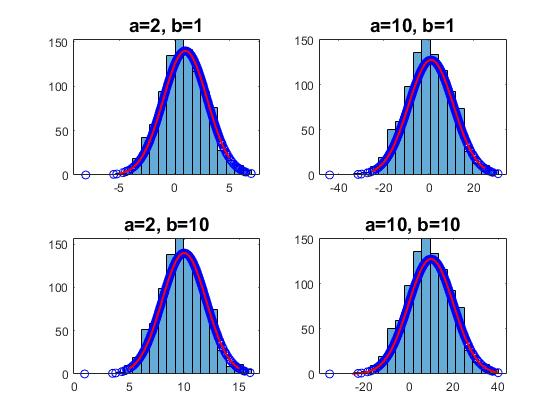
\includegraphics[width=\linewidth]{2linear}
  \caption{Histogram plot of transforming a Gaussian kernel $\mathcal{N}(0,1)$ by $f(x)=ax+b$ with sample size 1000}
  \label{fig:2linear}
\end{figure}

Starting with the distribution $X\sim\mathcal{N}(0,1)$ and performing the transformation Y=aX+b leads to the distribution plotted in figure \ref{fig:2linear}. This is the distribution $Y\sim\mathcal{N}(a\mu+b,\sigma^2a^2)=\mathcal{N}(b,a^2)$. The derivation for this can be seen in equations \ref{eq:2linearder}. Figure \ref{fig:2linear} shows the histogram data for a sample of 1000 variables in addition to each variable being transformed individually using the Jacobian to form the dotted distribution shown. 

\begin{equation}
\label{eq:2linearder}
\begin{split}
&f(X)=aX+b\\
&J=|f'(x)|=|a|\\
&p(y) = \sum_{1}^{1} \frac{p(x)}{J} = \frac{p(\frac{y-b}{a})}{|a|} \\
&p(y)=\frac{1}{a\sigma\sqrt{2\pi}}exp(-\frac{1}{2}[\frac{y-b-a\mu}{a\sigma}]^2)\\
&Y\sim\mathcal{N}(a\mu+b,a^2\sigma^2)\\
\end{split}
\end{equation} 

\begin{figure}[h]
  \centering
    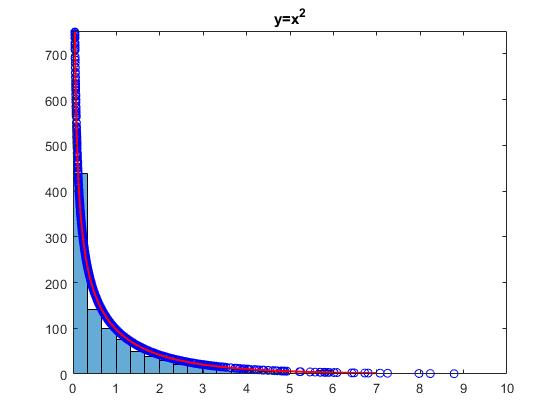
\includegraphics[width=\linewidth]{2quadratic}
  \caption{Histogram plot of transforming a Gaussian kernel $\mathcal{N}(0,1)$ by $f(x)=x^2$ with sample size 1000}
  \label{fig:2quadratic}
\end{figure}

The transformation $Y=X^2$ was applied to another Gaussian distribution following $X\sim\mathcal{N}(0,1)$. Figure \ref{fig:2quadratic} shows the result of this. The distribution $p(y)=\frac{1}{\sqrt{y2\pi}}exp(-\frac{1}{2}y)$ is overlain. This distribution was calculated using the same Jacobian method and is shown in equations \ref{eq:2quadraticder}. As $Y=X^2$ is not a 1:1 function the derivation required summing over all possible y values for a given x.


\begin{equation}
\label{eq:2quadraticder}
\begin{split}
&f(X)=X^2\\
&J=|f'(x)|=2|X|=2\sqrt{y}\\
&p(y) = \sum_{1}^{2} \frac{p(x)}{J} = \frac{p(+\sqrt{y})+p(-\sqrt{y})}{2\sqrt{y}}\\
&p(y)=\frac{p(\sqrt{y}))}{\sqrt{y}}\: by\:symmetry\\
&p(y)=\frac{1}{\sigma\sqrt{y2\pi}}exp(-\frac{1}{2}[\frac{\sqrt{y}-\mu}{\sigma}]^2)\\
&\:\sigma=1,\:\mu=0\\ 
\end{split}
\end{equation} 



\subsubsection{Matlab code} %-------------------------
The Matlab code for the transformation Y=aX+b can be seen in section 2.0 of the appendix, the transformation $Y=X^2$ is shown in section 2.1.

%---------------------------------------------------
\subsection{3. Inverse CDF method}
\begin{figure}[h]
  \centering
    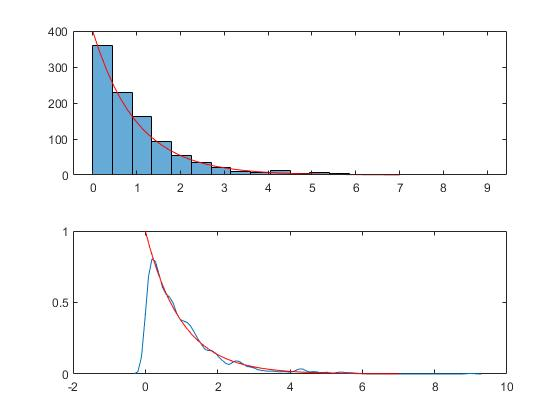
\includegraphics[width=\linewidth]{3exp}
  \caption{Histogram and kernel density plot of an exponential distribution generated using the inverse CDF method on a uniform kernel $\mathcal{U}(0,1)$ with sample size 1000}
  \label{fig:3exp}
\end{figure}
 
\begin{equation}
\label{eq:3cdf}
\begin{split}
&CDF = \int_0^yp(y)dy=\int_0^ye^{-y}\\
&CDF = 1- e^{-y} = F(y)\\
&F^{-1}(y) = -ln(1-y)\\
\end{split}
\end{equation} 

\begin{figure*}[h]
  \centering
    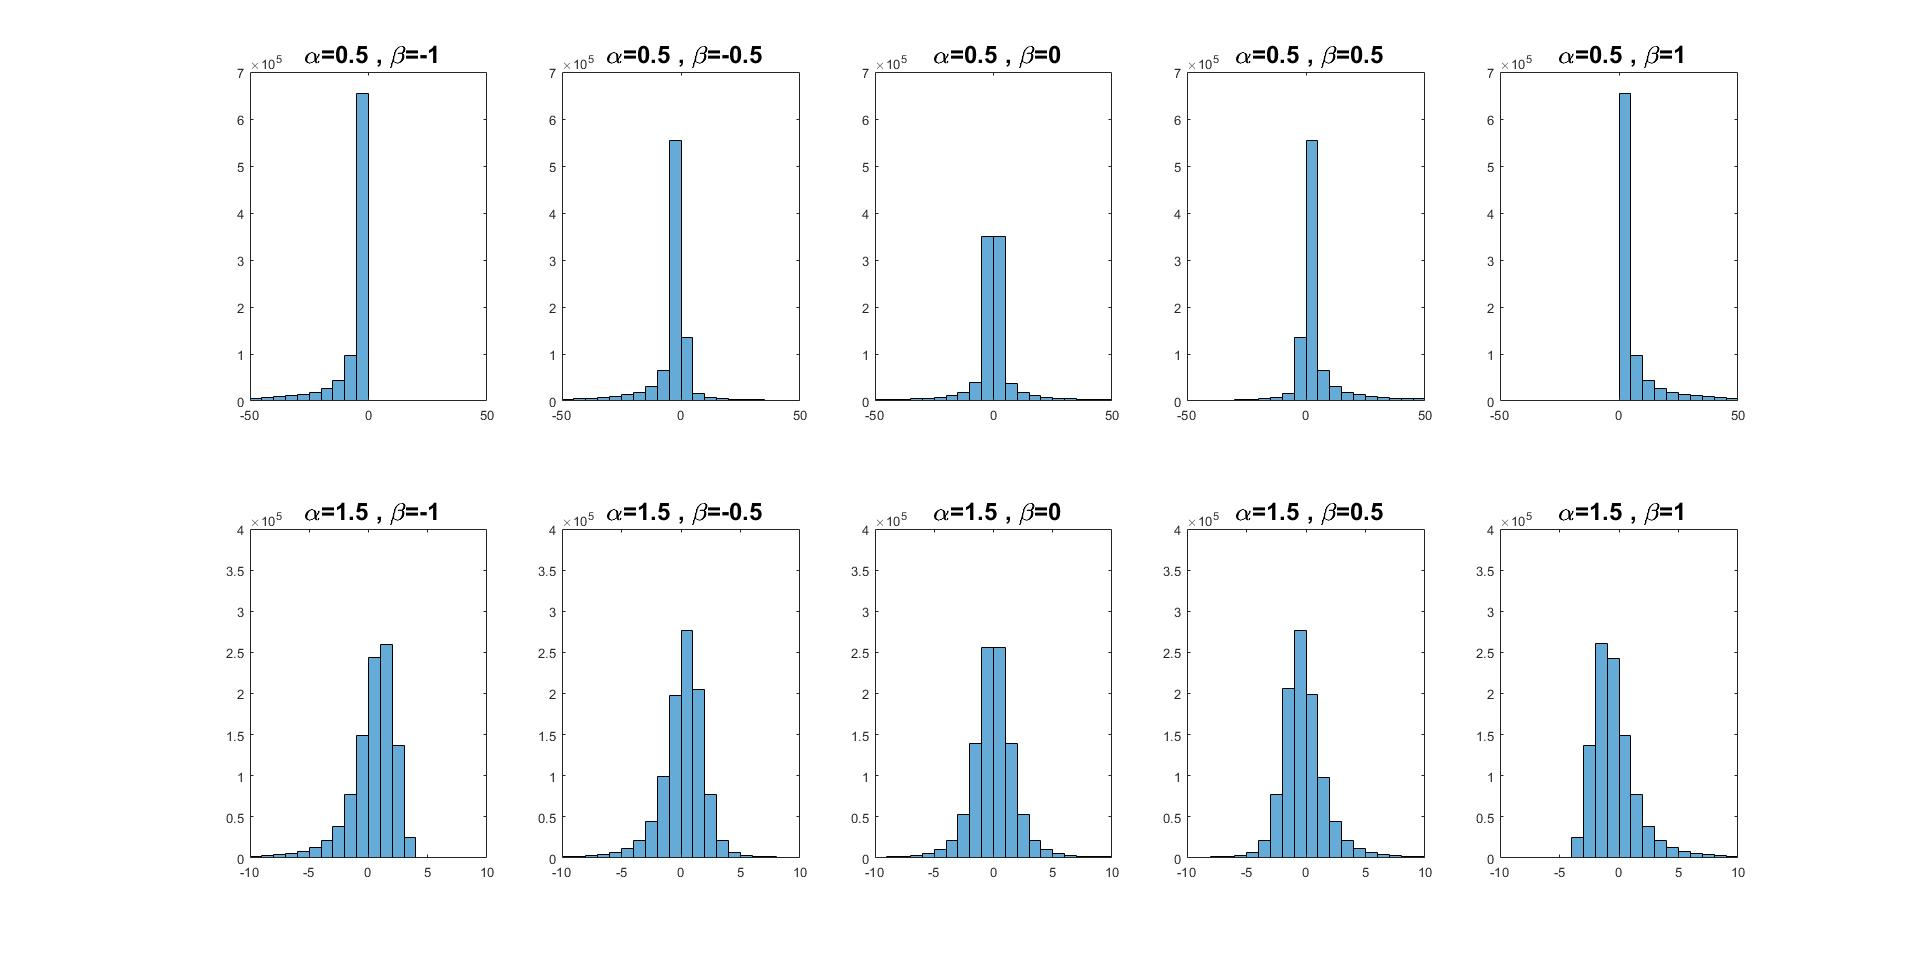
\includegraphics[width=\textwidth ]{4dist}
  \caption{Histogram plots of distribution X in equation \ref{eq:4equ} using various values for constants a and b, all from the same kernels $\mathcal{U}(-\frac{\pi}{2},\frac{\pi}{2})$ and $\mathcal{E}(1)$ with sample size 1000.}
  \label{fig:4dist}
\end{figure*}

The cumulative distribution function (CDF) for an exponential distribution p(y) = $e^{-y}$ is calculated in equations \ref{eq:3cdf}. Though the use of the inverse CDF and equation \ref{eq:3gen} an exponentially distributed random variable can be generated using a uniform kernel $\mathcal{U}(0,1)$. This generated distribution is shown in figure \ref{fig:3exp} with p(y) overlain. The curves match up with great accuracy especially the kernel density plot. This shows the validity of this method in generating different random variable densities.    

\begin{equation}
\label{eq:3gen}
y^{i} = F^{-1}(x^i)
\end{equation}

\subsubsection{Matlab code} %-------------------------
The Matlab code for the inverse CDF method can be seen in section 3.0 of the appendix.

%---------------------------------------------------
\subsection{4. Simulation from a 'difficult' density}




By using the non linear transformation listed in equations \ref{eq:4equ} and various values for $\alpha$ and $\beta$ the graphs in figure \ref{fig:4dist} can be produced. These graphs indicate that as $\alpha$ approaches 2 the distribution approaches normal, with a more rounded central peak. A low $\alpha$ such as 0.5 results in a very sharp density peak at 0. $\beta$ appears to affect the skew of the distribution. A negative $\beta$ results in negative skew and vice versa. 


\begin{equation}
\label{eq:4equ}
\begin{split}
&\alpha \in (0,2) \: \beta \in [-1,1]\\
&b=\frac{1}{\alpha}tan^{-1}(\beta tan(\frac{\pi\alpha}{2}))\\
&s=(1+\beta^2tan^2(\frac{\pi\alpha}{2}))^{\frac{1}{2\alpha}}\\
&U\sim\mathcal{U}(-\frac{\pi}{2},\frac{\pi}{2})\:V\sim\mathcal{E}(1)\\
& X=s\frac{sin(\alpha(U+b))}{(cosU)^{1/\alpha}}%(\frac{cos(U-\alpha(U+b))}{V})^{\frac{1-\alpha}{\alpha}}\\
\end{split}
\end{equation}

\subsubsection{Matlab code} %-------------------------
The Matlab code for this transformation can be seen in section 4.0 of the appendix.


%---------------------------------------------------
%------------------------------------------------

\section{Appendix}
\begin{large}
1.0 Uniform and normal random variables
\end{large}
\newline
\begin{itshape}
\%Plot Normal Distributions\\
figure(1)\\
x=randn(1000,1);\\
subplot(211),\\
histogram(x,20)\\
hold on\\
n = [-3:.1:3];\\
norm = normpdf(n,0,1)*350;\\
plot(n,norm,'red')\\
hold off\\
subplot(212),\\
ksdensity(x,'width',0.1)\\
hold on\\
n = [-3:.1:3];\\
norm = normpdf(n,0,1);\\
plot(n,norm,'red')\\
hold off\\

\%plot Uniform Distribution\\
figure(2)\\
y=rand(1000,1);\\
subplot(211),\\
histogram(y,10)\\
axis([0 1 0 150])\\
hold on\\
height = 100.* ones(length(n),1)\\
plot(n,height,'red')\\
hold off\\
subplot(212),\\
ksdensity(y,'width',0.1)\\
hold on\\
x1=[0,0,1,1];\\
y1=[0,1,1,0];\\
plot(x1,y1,'red')\\
hold off\\

\%plot Uniform no.2 Distribution\\
N=[100,1000,10000]\\
height=[20,150,1200]\\
figure(3)\\
for i =1:3 \\
	y=rand(N(i),1);\\
	subplot(3,1,i),\\
	histogram(y,10)\\
	title(['N=',num2str(N(i))])\\
	hold on\\
	mean=N(i)*0.1;\\
	sd= sqrt(N(i)*0.1*0.9);\\
	line([0,1],[mean,mean],'color','red')\\
	line([0,1],[mean+3*sd,mean+3*sd],'color','red')\\
	line([0,1],[mean-3*sd,mean-3*sd],'color','red')\\
	axis([0 1 0 height(i)])\\
	hold off\\
end\\
\end{itshape}

\begin{large}
2.0 Transforming a Gaussian by Y=aX+b
\end{large}
\newline
\begin{itshape}
x=randn(1000,1);\\
a=2;\\
b=1;\\
y=a*x+b;\\
J=abs(a);\\

py=0;\\
for i = 1:1 \%only one possible value for x given y\\
    py = normpdf((y-b)/a,0,1)/J ;\\
end\\
    
\%Plot Transformed Distributions\\
figure(1)\\
subplot(221),\\
histogram(y,20)\\
hold on\\
scatter(y,py*700,'blue')\\
f = @(x) 1/(sqrt(2*pi)*a) *exp(-0.5*(x-b)\^2/(a\^2)) *700\\
fplot(f,[-5,5],'red','LineWidth',1.5)\\
hold off\\
title('\textbackslash fontsize\{14\} a=2, b=1')\\

subplot(222),\\
a=10;\\
b=1;\\
y=a*x+b;\\
J=abs(a);\\
py=0;\\
for i = 1:1 \%only one possible value for x given y\\
    py = normpdf((y-b)/a,0,1)/J ;\\
end\\
histogram(y,20)\\
hold on\\
scatter(y,py*3200,'blue')\\
f = @(x) 1/(sqrt(2*pi)*a) *exp(-0.5*(x-b)\^2/(a\^2)) *3200\\
fplot(f,[-25,25],'red','LineWidth',1.5)\\
hold off\\
title('\textbackslash fontsize\{14\} a=10, b=1')\\

subplot(223),\\
a=2;\\
b=10;\\
y=a*x+b;\\
J=abs(a);\\
py=0;\\
for i = 1:1 \%only one possible value for x given y\\
    py = normpdf((y-b)/a,0,1)/J ;\\
end\\
histogram(y,20)\\
hold on\\
scatter(y,py*700,'blue')\\
f = @(x) 1/(sqrt(2*pi)*a) *exp(-0.5*(x-b)\^2/(a\^2)) *700\\
fplot(f,[5,15],'red','LineWidth',1.5)\\
hold off\\
title('\textbackslash fontsize\{14\} a=2, b=10')\\

subplot(224),\\
a=10;\\
b=10;\\
y=a*x+b;\\
J=abs(a);\\
py=0;\\
for i = 1:1 \%only one possible value for x given y\\
    py = normpdf((y-b)/a,0,1)/J ;\\
end\\
histogram(y,20)\\
hold on\\
scatter(y,py*3200,'blue')\\
f = @(x) 1/(sqrt(2*pi)*a) *exp(-0.5*(x-b)\^2/(a\^2)) *3200\\
fplot(f,[-25,40],'red','LineWidth',1.5)\\
hold off\\
title('\textbackslash fontsize{14} a=10, b=10')\\

\end{itshape}

\begin{large}
2.1 Transforming a Gaussian by $Y=X^2$
\end{large}
\newline
\begin{itshape}
x=randn(1000,1);\\
y=x.\^{}2;   \\
py=zeros(length(y),1);\\
for i = 1:2 \%y=x\^{}2 is a 2:1 function\\
    J=abs(x)*2;\\
    py = py + normpdf((-1)\^{}i*sqrt(y),0,1)./J ;\\
end\\

\%Plot Transformed distribution\\
figure(1)\\
histogram(y,40)\\
hold on\\
scatter(y,py*400,'blue')\\
f = @(x) 1/(sqrt(2*pi*x)) *exp(-0.5*(sqrt(x))\^{}2) *400\\
fplot(f,[0,7],'red','LineWidth',1.5)\\
hold off\\
title('y=x\^{}2')\\
axis([0 10 0 750])\\
\end{itshape}

\begin{large}
3.0 Generating an exponential distribution using CDF method
\end{large}
\newline
\begin{itshape}
x=rand(1000,1);\\
y= -log(-x+1);\\

figure(1)\\
subplot(211),\\
histogram(y,20);\\
hold on \\
f = @(x) 400*exp(-x)\\
fplot(f,[0,7],'red')\\
hold off\\
subplot(212),\\
ksdensity(y,'width',0.1)\\
hold on \\
f = @(x) exp(-x)\\
fplot(f,[0,7],'red')\\
hold off\\
\end{itshape}


\begin{large}
4.0 Simulation from a difficult density
\end{large}
\newline
\begin{itshape}
v=exprnd(1,1000,1);\\
u=rand(1000,1);\\
u=(u-0.5)*pi ;\\
alpha=0.5;\\
betavals=[-1,-0.5,0,0.5,1,-1,-0.5,0,0.5,1];\\
x=zeros(length(u),10);\\

figure(1)\\
histrange=50;\\
range=700;\\

for i = 1:10\\
beta = betavals(i);\\
if i>5\\
    alpha = 1.5;\\
    histrange=10;\\
    range=400;\\
end \\
b=1/alpha * atan(beta*tan(pi*alpha/2)) ;\\
s=(1+beta\^{}2*(tan(pi*alpha/2))\^{}2)\^{}(1/(2*alpha));\\
x(:,i)=s* sin(alpha*(u+b))./(cos(u).\^{}(1/alpha)).* (cos(u-alpha*(u+b))./v).\^{}((1-alpha)/alpha); \\
subplot(2,5,i),\\
histogram(x(:,i),[-histrange:histrange/10:histrange])\\
axis([-histrange histrange 0 range])\\
tit = strcat('\textbackslash fontsize\{18\} \textbackslash alpha=',num2str(alpha), '\textbackslash fontsize\{18\} , \textbackslash beta=',num2str(beta));\\
title(tit)\\
end\\
\end{itshape}




%------------------------------------------------
\end{document}
